\begin{minipage}[c]{\textwidth}
\advance\leftskip-2.5cm
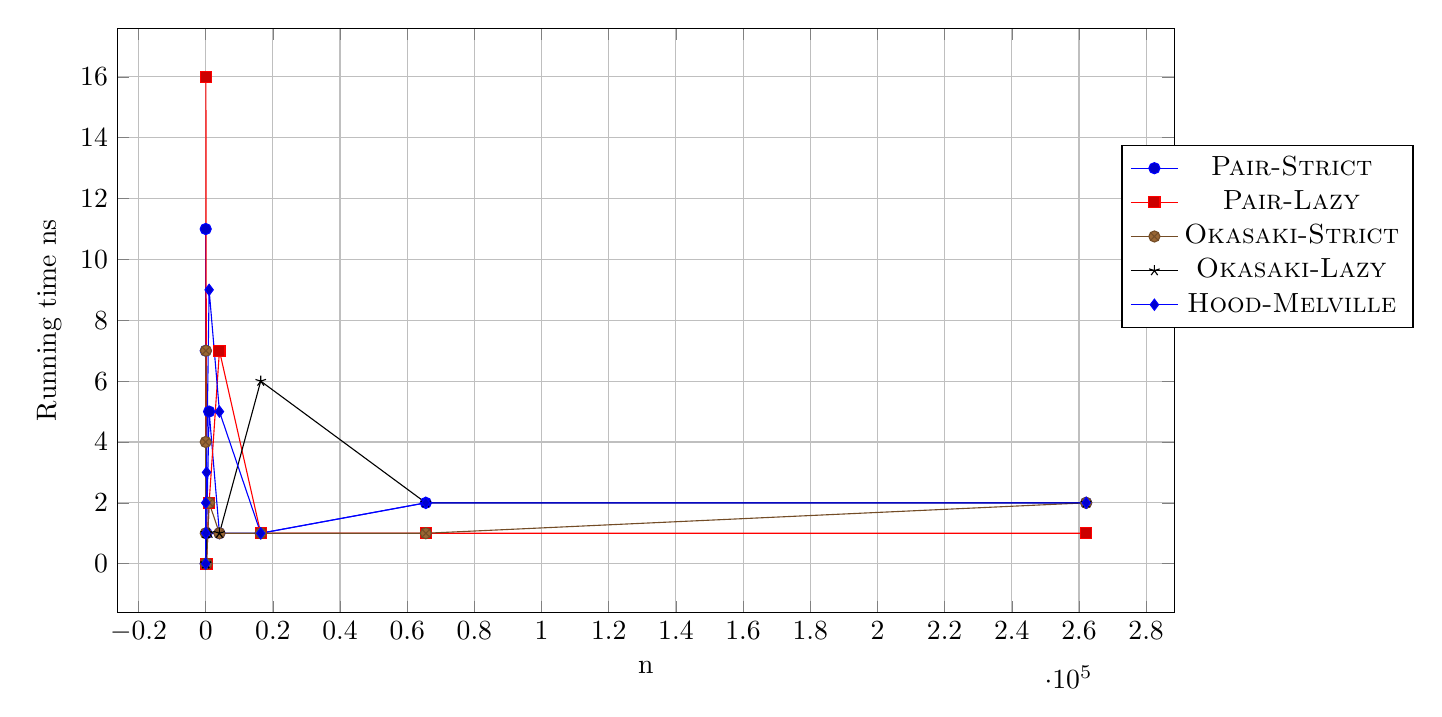
\begin{tikzpicture}
        \begin{axis}[
            xlabel = n,
            ylabel = Running time ns,
            height=9cm,
            width=15cm,
            grid=major,
            legend style={
            at={(0.95,0.8)},
            anchor=north west}]            
            legend pos=center west
    	]
    		
  
                \addplot coordinates {
(2,11)
(4,0)
(16,7)
(64,0)
(256,1)
(1024,5)
(4096,1)
(16384,1)
(65536,2)
(262144,2)

    	};
        
    	\addlegendentry{\textsc{Pair-Strict}}

        \addplot coordinates {
(2,0)
(4,0)
(16,0)
(64,16)
(256,0)
(1024,2)
(4096,7)
(16384,1)
(65536,1)
(262144,1)

    	};
        
    	\addlegendentry{\textsc{Pair-Lazy}}

        \addplot coordinates {
(2,4)
(4,0)
(16,1)
(64,7)
(256,0)
(1024,2)
(4096,1)
(16384,1)
(65536,1)
(262144,2)

    	};
        
    	\addlegendentry{\textsc{Okasaki-Strict}}

        \addplot coordinates {
(2,1)
(4,0)
(16,0)
(64,0)
(256,1)
(1024,1)
(4096,1)
(16384,6)
(65536,2)
(262144,2)

    	};
        
    	\addlegendentry{\textsc{Okasaki-Lazy}}

        \addplot coordinates {
(2,1)
(4,0)
(16,2)
(64,1)
(256,3)
(1024,9)
(4096,5)
(16384,1)
(65536,2)
(262144,2)

    	};

    	\addlegendentry{\textsc{Hood-Melville}}

        \end{axis}

    \end{tikzpicture}
    \captionof{figure}{Total time of Breadt-First search for a complete binary tree divided by the number of nodes in the tree}
    \label{fig:sample_figure}
\end{minipage}
